\section{The Proposed H-SFP Framework}
\label{sec:methodology}
\begin{figure}[ht]
    \centering
    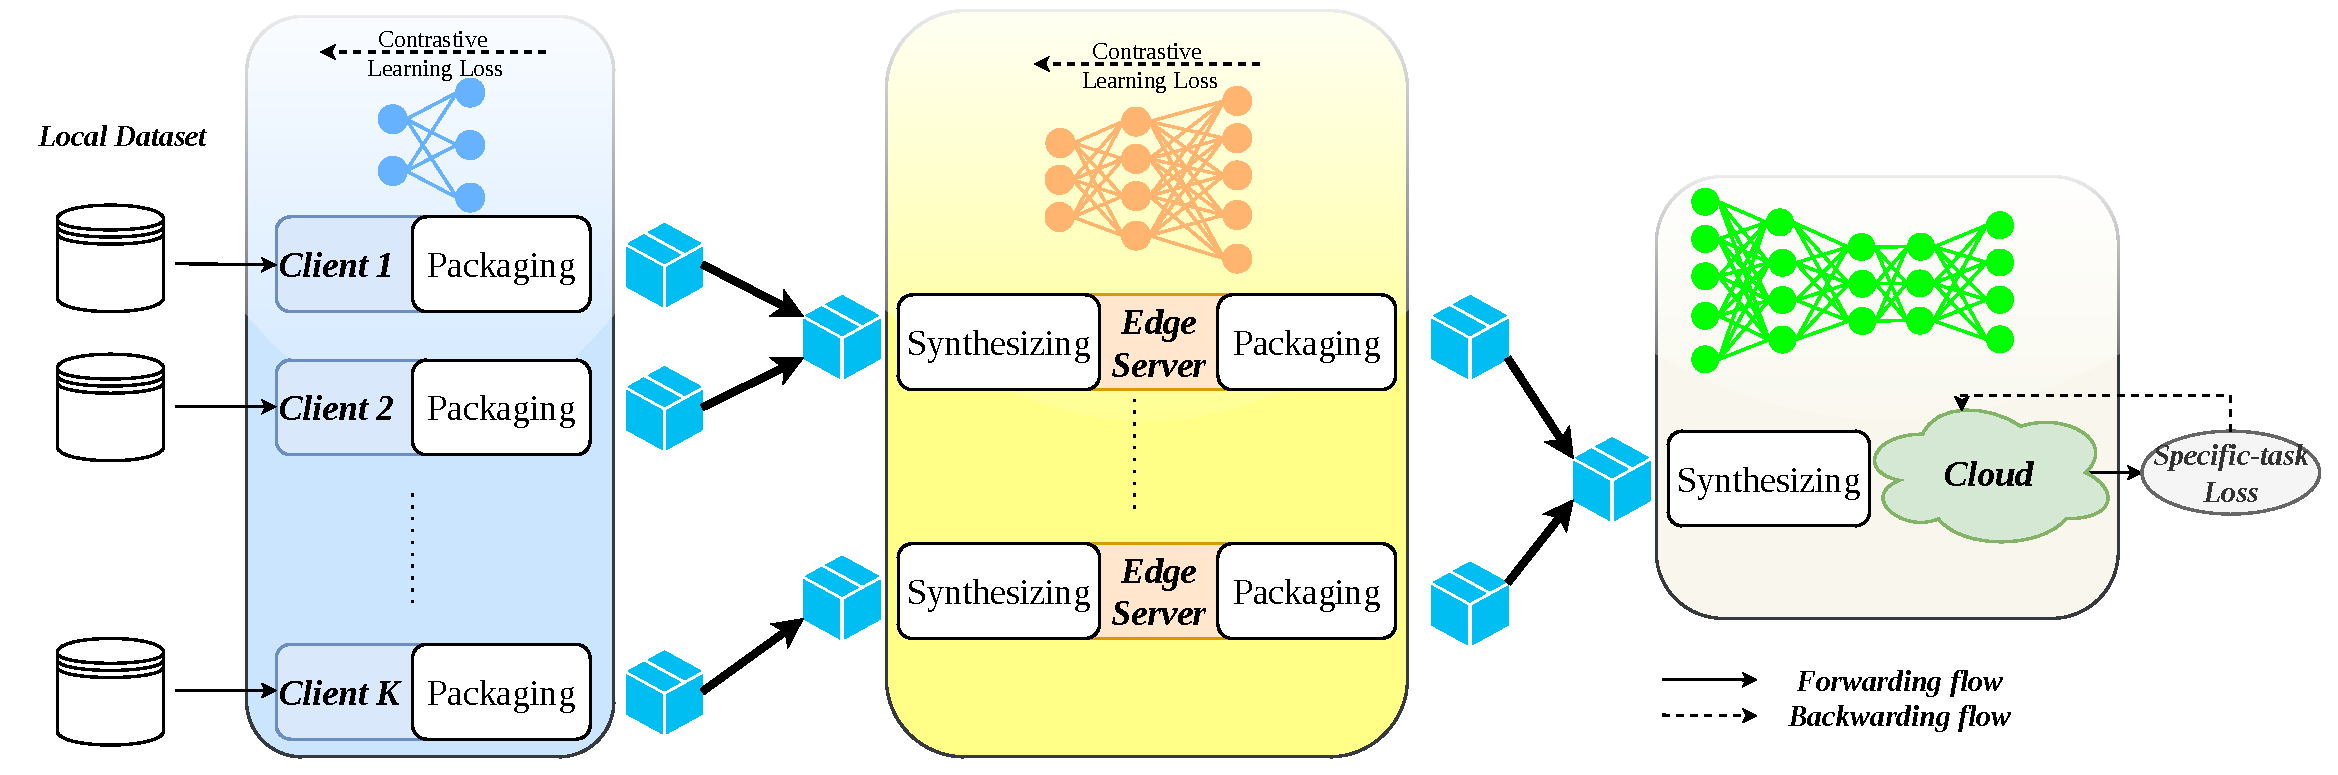
\includegraphics[width=\linewidth]{
    Figures/method-2.pdf}
    \caption{The H-SFP architecture and data flow. Clients communicate class-wise feature statistics instead of sample-level activations and gradients. Edge and cloud tiers iteratively aggregate statistics, synthesize feature distributions, and train their assigned model components.}
    \label{fig:method-p2}
\end{figure}
\begin{figure}[t]
    \centering
    \begin{subfigure}{0.44\linewidth}
        \centering
        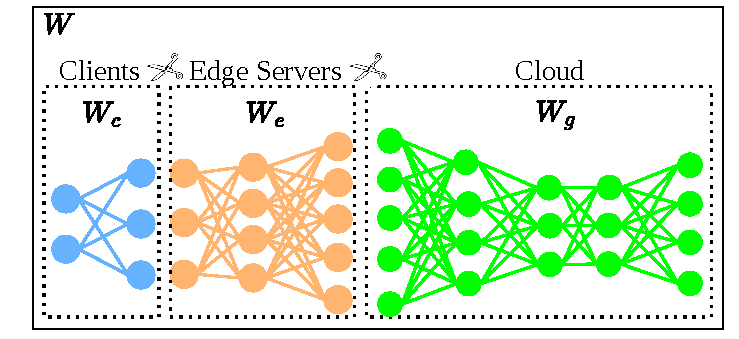
\includegraphics[width=\linewidth]{Figures/method-3.pdf}
        \caption{Hierarchical Model Partitioning.}
        \label{fig:method-p3}
    \end{subfigure}
    \hfill
    \begin{subfigure}{0.54\linewidth}
        \centering
        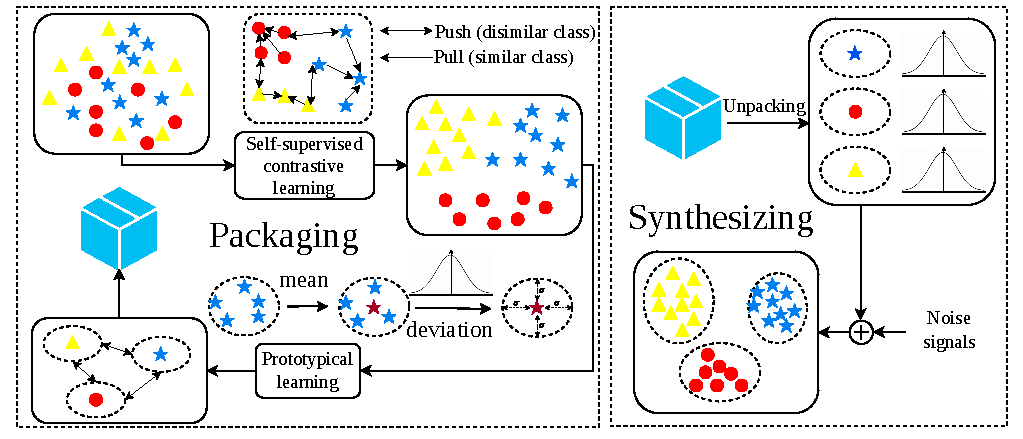
\includegraphics[width=\linewidth]{Figures/method-1.pdf}
        \caption{Generative Prototyping.}
        \label{fig:method-p1}
    \end{subfigure}
    \caption{The proposed H-SFP Framework. (a) Model partitioning ($W_c, W_e, W_g$) offloads computational burden from the clients. (b) The core generative prototyping mechanism, where self-supervised contrastive learning at the client level enables the compression of representations into lightweight statistical moments ($\mu$, $\sigma$).}
    \label{fig:h_sfp_framework_combined}
\end{figure}
We propose H-SFP, which replaces cross-tier backpropagation with statistic-based feature synthesis. Each tier trains its assigned model part locally, packages its learned feature distribution into lightweight class-wise statistics, and transmits only these statistics upward. The following subsections describe the system architecture, prototype packaging and synthesis, and the resulting communication behavior. 
Concrete algorithms for each tier are provided in the Appendix~B.

\subsection{System Architecture and Motivation}
\label{subsec:system_model}
We consider a three-tier ``cloud-edge-client'' framework shown in~\Cref{fig:method-p2}, comprising a global cloud server, $M$ edge servers, and $K$ clients partitioned into $M$ disjoint clusters $\{\mathcal{C}_m\}_{m=1}^M$. This framework directly addresses the scalability bottleneck of centralized FL by allowing edge servers to perform intermediate aggregations. In real-world deployments, this partitioning would be determined by physical proximity or by network latency pinging. However, for our empirical evaluation, we deliberately adopt a random assignment strategy. This represents a strict, unoptimized baseline, demonstrating that H-SFP's generative aggregation can successfully stabilize distributions and mitigate client drift even without the benefit of a geographically optimized or clustered network topology.

To solve resource-constrained clients, H-SFP adopts a split-learning architecture. As illustrated in \Cref{fig:method-p3}, the global model $W$ is partitioned into three components: a lightweight client-side feature extractor $W_c$, an intermediate edge-side model $W_e$, and a cloud-side task model $W_g$. This reduces the computational and memory burden on clients by offloading deeper network layers to upper tiers. However, conventional split federated learning requires continuous transmission of intermediate activations and gradients to maintain end-to-end optimization, leading to substantial communication and synchronization overhead.

H-SFP resolves this by replacing backpropagation with a feed-forward, multi-tier generative prototyping mechanism (\Cref{fig:method-p1}). By transmitting lightweight statistics rather than raw activations, we completely decouple the network segments, enabling communication-efficient and asynchronous training. Additionally, the precise cut points are treated as hyperparameters determined by the target device's memory constraints. For instance, clients may only compute the first residual block of a ResNet architecture, offloading the deeper, computationally expensive blocks to the edge and cloud tiers.

\subsection{Multi-tier Self-Learning} 
\label{sec:multi_tier_learning}
    
The first tier of learning occurs on resource-constrained clients. Each client $k$ trains its local extractor \textcolor{black}{$W_{c,k}$} using its private data $\mathcal{D}_k$. The objective $\mathcal{L}_k(W_{c,k})$ is to learn a robust representation space using the self-supervised NT-Xent contrastive loss \cite{chen2020simple}. For a batch $B$, let $z_i = W_{c,k}(x_i)$ where $x_i \in D_k$:
\begin{equation}
    \label{eq:supcon}
    \mathcal{L}_{k}(W_{c,k})= \mathcal{L}_{\text{con}, k} = \sum_{i\in B}\frac{-1}{|P(i)|}\sum_{p\in P(i)}\log\frac{\exp(z_{i}\cdot z_{p}/\tau)}{\sum_{a\in A(i)}\
    exp(z_{i}\cdot z_{a}/\tau)}
\end{equation}
where $A(i)$ is the set of other samples in the batch, $P(i)$ contains positive samples sharing the same class label as $i$, and $\tau$ is a temperature scalar. After training, the client distills its feature space into class-conditional statistics.
At the second tier, the edge server $m$ operates without access to real data. It aggregates the statistics $\{\mu_k, \sigma_k\}$ from its client cluster $\mathcal{C}_m$ to form a stable distribution $(\mu_m, \sigma_m)$. The edge server $m$ unpacks these statistics to synthesize a new feature dataset, $D^{syn}_m$, which serves as the input for the edge-side part $W_{e,m}$. $W_{e,m}$ is trained using the same contrastive objective on its own outputs, $\mathcal{L}_m(W_{e,m}) = \mathcal{L}_{\text{con}, m}(W_e(D_{syn}^{\text{edge}}))$. Enforcing consistency across tiers ensures that $W_e$ learns relative structural relationships rather than overfitting to synthetic noise.

Finally, the cloud tier aggregates the class-conditional feature statistics from all $M$ edge servers to form a global synthetic dataset, $D_{\text{syn}}^{\text{global}}$. The aggregated means and standard deviations are used to sample representative feature embeddings for each class. The task-specific part $W_g$ is then trained on this synthesized dataset using the standard supervised loss $\mathcal{L}_g(W_g) = \mathcal{L}_{\text{task}}\big(W_g(D_{syn}^{\text{global}})\big)$.

\subsection{Dual-Timescale Transmission and Augmentation}
\label{sec:transmission_augmentation}
Our communication mechanism operates on a dual-timescale to balance efficiency with long-term stability. At the fast timescale, clients transmit only their class-wise prototype statistics, including the local $\mu_{k}^{(j)}$ and $\sigma_{k}^{(j)}$ of class $j$:
\begin{equation}
    \mu_k^{(j)} = \frac{1}{|\mathcal{D}_k^{(j)}|} \sum_{x_i \in \mathcal{D}_k^{(j)}} W_{c,k}(x_i), \quad
    \sigma_k^{(j)} = \sqrt{\frac{1}{|\mathcal{D}_k^{(j)}|} \sum_{x_i \in \mathcal{D}_k^{(j)}} (W_{c,k}(x_i) - \mu_k^{(j)})^2}.
    \label{mean_std_client}
\end{equation}
This drastically reduces overhead to $O(J_k \times d_c)$ per client, where $J_k$ is the class count and $d_c$ the feature dimension. Infrequently (slow timescale interval $I_c$), a standard model averaging of $W_{c,k}$ occurs to correct long-term client drift. 

Upon receiving \textcolor{black}{($\mu_k$, $\sigma_k$)}, the edge server synthesizes features $z_{syn}$ for class $j$ by sampling from a multivariate Gaussian as in \cite{9578909,Nguyen_2026_CVPR} as follows:
\begin{equation}
    \label{eq:synthesis}
    z_{syn} \sim \mathcal{N}\big(\mu_m^{(j)}, \text{diag}(\sigma_m^{(j)} + \epsilon)^2\big)
\end{equation}
where $\text{diag}(\cdot)$ creates a diagonal covariance matrix and $\epsilon$ ensures numerical stability. We intentionally restrict the synthesis to a diagonal covariance matrix to achieve an optimal trade-off. Transmitting a full covariance matrix would increase the communication cost to $O(d_c^2)$, recreating the SL bottleneck. However, our ablation studies in \Cref{sec:ablation} confirm that transmitting per-dimension variance ($\sigma$) rather than just the mean ($\mu$) is critical for capturing the elliptical boundaries of feature clusters. Unlike SFL, which transmits exact, invertible activation maps for every sample, H-SFP transmits aggregated, class-wise statistics that obfuscate individual features, serving as a natural defense against feature-space inversion attacks while remaining semantically rich.

\subsection{Theoretical Justification: Information Preservation}
\label{sec:mmd_theory}
    
A fundamental concern with generative prototyping is the potential loss of high-rank structural information when replacing raw activations with $(\mu, \sigma)$. We theoretically bound this distribution shift between the true client representations $H_{true}$ and the edge-synthesized features $\hat{H}_{gen}$ using Maximum Mean Discrepancy (MMD). Let $\mathcal{X}$ be the feature space defined by $W_c$. Given a characteristic kernel $k: \mathcal{X} \times \mathcal{X} \rightarrow \mathbb{R}$ mapping to a Reproducing Kernel Hilbert Space (RKHS), the empirical MMD between the true feature distribution $\mathbb{P}$ and the synthesized Gaussian distribution $\mathbb{Q}$ is bounded by: 
\begin{equation}
\label{eq:mmd_bound}
\text{MMD}^2(\mathbb{P}, \mathbb{Q}) = \mathbb{E}_{x, x' \sim \mathbb{P}}[k(x, x')] + \mathbb{E}_{y, y' \sim \mathbb{Q}}[k(y, y')] - 2\mathbb{E}_{x \sim \mathbb{P}, y \sim \mathbb{Q}}[k(x, y)].
\end{equation}

To ensure $\text{MMD}^2(\mathbb{P}, \mathbb{Q}) \to 0$ and that the synthesized geometry preserves the semantic manifold, we introduce a statistical constraint on the feature extractor. 

\noindent\textbf{Assumption 1 (Feature-Space Lipschitz Continuity):} There exists a constant $L_{stat} > 0$ such that for any two data samples $x_1, x_2$, the divergence of their generated prototype statistics is bounded by the input space distance:
\begin{equation}
\label{eq:lipschitz}
||\mu(x_1) - \mu(x_2)||_2 + ||\sigma(x_1) - \sigma(x_2)||_2 \leq L_{stat} ||x_1 - x_2||_2.
\end{equation}
By enforcing Assumption 1 during local client updates via the contrastive loss, the divergence between the actual and synthesized manifolds remains strictly bounded across aggregation rounds, preventing information loss.

\subsection{Asymptotic Convergence Analysis}
\label{sec_convergence_analysis}

Establishing end-to-end convergence guarantees for the H-SFP topology requires departing from standard federated optimization proofs. Because our framework decouples the computational tiers, optimization at the upper tiers is performed over a dynamically shifting probability measure space parameterized by the tier below. To bound this shifting measure, we adopt standard stochastic non-convex assumptions along with a novel measure-theoretic constraint.

\noindent\textit{Assumption 2 (Measure Theoretic Lipschitz Continuity).} Let $\mathcal{P}(\mathcal{Z})$ denote the space of synthesized prototype measures. The expected loss functional $\mathcal{L}$ is $L_{m}$ Lipschitz continuous with respect to the Wasserstein 2 distance $\mathcal{W}_2$ between generated distributions $\mathbb{Q}_1, \mathbb{Q}_2 \in \mathcal{P}(\mathcal{Z})$:
\begin{equation}
|\mathbb{E}_{z \sim \mathbb{Q}_1}[\mathcal{L}(W; z)] - \mathbb{E}_{z \sim \mathbb{Q}_2}[\mathcal{L}(W; z)]| \le L_{m} \cdot \mathcal{W}_2(\mathbb{Q}_1, \mathbb{Q}_2).
\end{equation}

\noindent\textit{Assumption 3 (Bounded Variances and Second Moments).} The variance and second moments of stochastic gradients for each layer $l$ have upper bounds, denoted by $\sigma_l^2$ and $G_l^2$, respectively.
Operating under these constraints, we formally establish the global convergence of the decoupled architecture. The rigorous measure-theoretic derivation is deferred to the Appendix~C.

\noindent\textit{Theorem 1 (Asymptotic Convergence of H-SFP).} Under standard non-convex assumptions and Assumptions 2 and 3, the decoupled parameters asymptotically converge to a bounded stationary neighborhood. Specifically, for the global classifier $W$ optimized over $R$ total communication rounds with learning rate $\eta$, local aggregation intervals $I_m$, and layer split boundaries $L_m$, the expected gradient norm satisfies
\begin{multline}
\frac{1}{R}\sum_{t=1}^{R}\mathbb{E}[||\nabla \mathcal{L}(\overline{W}^{t-1})||_2^2] \le \frac{2\Delta}{\eta R} + \frac{L\eta\sum_{l=1}^{L_{\mathrm total}} \sigma_l^2}{N} \\ + 4L^2\eta^2\sum_{m=1}^{M-1}\left(\mathbb{I}_{\{I_m>1\}}I_m^2\sum_{l=L_{m-1}+1}^{L_m} G_l^2\right)
\end{multline}
where $\Delta = \mathcal{L}(\overline{W}^0) - \mathcal{L}^*$, and $\mathbb{I}_{\{\cdot\}}$ is the indicator function.

\noindent\textit{Proof Sketch (Hierarchical Measure Stabilization).} The proof proceeds inductively across the hierarchy. The induction initiates at the client tier, where the local extractors converge modulo standard SGD dynamics. The divergence between the aggregated sub-model and local sub-models is strictly bounded by the aggregation interval $I_m$ and the second moments $G_l^2$. Given $L_f$ Lipschitz embeddings, the sequence of client output measures stabilizes, driving the expected parametric shift to zero. As the edge model $W_e$ optimizes over the synthesized measure $\mathbb{Q}_{e}^t$, its temporal update incurs a stochastic drift bounded by $\delta_m^t = L_{m} \cdot \mathcal{W}_2(\mathbb{Q}_{e}^{t+1}, \mathbb{Q}_{e}^t)$. Because the underlying client-tier measures have stabilized, this drift term rigorously decays $\delta_m^t \to 0$, guaranteeing that $W_e$ converges to a stationary neighborhood despite the non-stationary nature of its input. Applying identical inductive logic to the cloud tier, the stabilization of the edge measures guarantees the convergence of the global synthetic distribution.